%  ClockGating.tex
%  Document created by seblovett on seblovett-Ubuntu
%  Date created: Sat 22 Feb 2014 13:20:20 GMT
%  <+Last Edited: Sat 22 Mar 2014 14:40:49 GMT by seblovett on seblovett-Ubuntu +>

\subsection{Clock Gating}

\subsubsection{Theory}

The clock in a sequential circuit can consume 15-45\% of the power \cite{pedram1996power}.
Therefore it is a large area of potential power saving.
Clock gating is an approach of controlling the clock to individual modules of a design by either stopping or slowing down the clock with respect to a master clock \cite{841927}. 
An approach, seen in \cite{tellez1995activity}, involves stopping the clock to unused modules.

This method can be realised using two simple circuits seen in figures \ref{fig:cg:circuit1} and \ref{fig:cg:circuit2}.
Although figure \ref{fig:cg:circuit1} is functionally complete, in reality, a latch is needed to remove any glitches in the circuit.
These are fundamentally different to load-enable registers, where the input is multiplexed between the current value or the input.
The load-enable registers are still clocked at the master clock frequency.

\begin{figure}
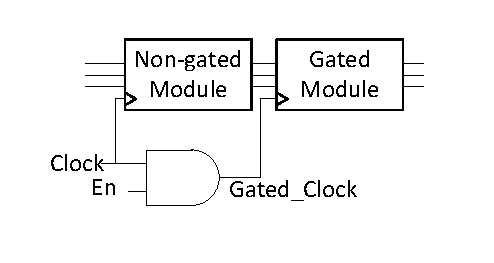
\includegraphics[width=0.5\textwidth]{Figures/clockgating_and.pdf}
\caption{Clock gating circuit using an \texttt{AND} gate}
\todo[inline]{Gated Module or Gated Circuit? Consistency with the other diagrams}
\todo[inline]{Is this even needed?}
\label{fig:cg:circuit1}
\end{figure}

\begin{figure}
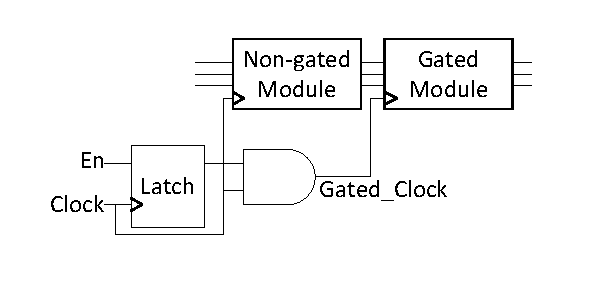
\includegraphics[width=0.5\textwidth]{Figures/clockgating_latch.pdf}
\caption{Clock gating circuit using an \texttt{AND} gate and a latch}
\todo[inline]{Gated Module or Gated Circuit? Consistency with the other diagrams}
\label{fig:cg:circuit2}
\end{figure}

\subsubsection{Synthesis Techniques}

A gating function is typically defined by the designer within the RTL design stage.
However, a more common approach is to allow the synthesis tool to obtain the gating functions from a gate-level netlist \cite{benini1999symbolic, hurst2008automatic}.

The general outline for the synthesis is to find the clock gating function for each flip-flop.
The flip-flops are then grouped so that they are driven by the same function. 
The problem of simplifying the gating function is looked at in \cite{han2012synthesis}. 
Here, an algorithm is suggested where the gating function is shared by existing combinational logic.
This was shown to reduce the logic added by introducing clock gating.

However, sometimes the addition of clock gating is not advantageous. 
The gating function can be large and therefore can cause timing violations, resulting in an unsuitable synthesis.
If the gating function is large enough, it can also consume more power than it saves.
Both of these issues are addressed in \cite{arbel2009resurrecting}.
Here, the author proposed solutions to large gating functions by reducing the depth of logic by an approximation. 
The approximation is made such that the resulting logic does not gate the clock more than the original function. 
It results in the flip-flop being clocked more often, but reduces the logic so that it can be utilised, thereby saving some power.
\cite{arbel2009resurrecting} also proposes the use of a clustering algorithm that looks at grouping similar gating functions. 
This can then reduce the overall logic needed to implement the clock gating and maximise the energy saved.

\subsubsection{Conclusion}

Clock gating is a simple principle to implement on a small scale.
The underlying theory is to disable a module when it is not in use.
This is done by identifying a gating function which disallows clock propagation if the function is asserted.

However, clock gating can produce large gating functions which violate the timing constraints of the circuit, or even consume more power than they save. This results in two problems that need solving - group formation and simplification \cite{han2012synthesis, paik2012clock}.







